%Created with command:
%"/home/josh/Teaching/trunk/Utilities/makeexam" "Homework 3 - Combinational Circuits" "Attempt the following problems.  Please show all of your work.  You may work with others however make sure that all work you submit is yours." "../CombinationalCircuits/Assessments/wakerly_4_6.tex" "../CombinationalCircuits/Assessments/wakerly_4_9.tex" "../CombinationalCircuits/Assessments/circuit_analysis_hw.tex" "../CombinationalCircuits/Assessments/wakerly_4_15.tex" "../CombinationalCircuits/Assessments/wakerly_4_36.tex"
%Modified to separate solutions onto multiple pages.
\documentclass{article}
\usepackage[T1]{fontenc}
\usepackage{arev}
\usepackage{longtable}
\usepackage[hmargin=2cm,vmargin=2cm]{geometry}
\usepackage{graphicx}
\setlength{\parindent}{0pt}
\title{Homework 3 - Combinational Circuits}
\date{}
\begin{document}
\maketitle
Attempt the following problems.  Please show all of your work.  You may work with others, however make sure that all work you submit is yours. (30 points total)
\begin{longtable}[l]{rp{17cm}}
%file: ../CombinationalCircuits/Assessments/wakerly_4_6.tex
1.&\begin{minipage}[t]{\linewidth}(6 pt) Do problem 4.6 in the text.\\ \\

Solution: \\ \\
(a)\\
\begin{tabular}{rll}
  $F$ & $= W \cdot X \cdot Y \cdot Z \cdot (W \cdot X \cdot Y \cdot Z' + W \cdot X' \cdot Y \cdot Z + W' \cdot X \cdot Y \cdot Z + W \cdot X \cdot Y' \cdot Z)$ &\\
      & $= W \cdot X \cdot Y \cdot Z \cdot W \cdot X \cdot Y \cdot Z' + W \cdot X \cdot Y \cdot Z \cdot W \cdot X' \cdot Y \cdot Z$ &\\ 
      & $\textrm{    }+ W \cdot X \cdot Y \cdot Z \cdot W' \cdot X \cdot Y \cdot Z + W \cdot X \cdot Y \cdot Z \cdot W \cdot X \cdot Y' \cdot Z$ & (T8)\\
      & $= W \cdot X \cdot Y \cdot Z \cdot Z' + W \cdot X \cdot Y \cdot Z \cdot X'+ W \cdot X \cdot Y \cdot Z \cdot W' + W \cdot X \cdot Y \cdot Z \cdot Y'$ & (T3')\\
      & $= 0 \cdot 0 \cdot 0 \cdot 0$ & (T5')\\
      & $= 0$ & (T2')\\
\end{tabular}\\ \\
Let the following be true:\\
\begin{tabular}{rl}
  $A$ & $= W \cdot X \cdot Y \cdot Z$\\
  $B$ & $= W \cdot X \cdot Y \cdot Z'$\\
  $C$ & $= W \cdot X' \cdot Y \cdot Z$\\
  $D$ & $= W' \cdot X \cdot Y \cdot Z$\\
  $E$ & $= W \cdot X \cdot Y' \cdot Z$\\
\end{tabular}\\ \\
Truth Table:\\
\begin{tabular}{cccc|ccccc|c}
  $W$ & $X$ & $Y$ & $Z$ & $A$ & $B$ & $C$ & $D$ & $E$ & \textbf{$F$}\\
  \hline
   0  &  0  &  0  &  0  &  0  &  0  &  0  &  0  &  0  & \textbf{ 0 }\\
   0  &  0  &  0  &  1  &  0  &  0  &  0  &  0  &  0  & \textbf{ 0 }\\
   0  &  0  &  1  &  0  &  0  &  0  &  0  &  0  &  0  & \textbf{ 0 }\\
   0  &  0  &  1  &  1  &  0  &  0  &  0  &  0  &  0  & \textbf{ 0 }\\
   0  &  1  &  0  &  0  &  0  &  0  &  0  &  0  &  0  & \textbf{ 0 }\\
   0  &  1  &  0  &  1  &  0  &  0  &  0  &  0  &  0  & \textbf{ 0 }\\
   0  &  1  &  1  &  0  &  0  &  0  &  0  &  0  &  0  & \textbf{ 0 }\\
   0  &  1  &  1  &  1  &  0  &  0  &  0  &  1  &  0  & \textbf{ 0 }\\
   1  &  0  &  0  &  0  &  0  &  0  &  0  &  0  &  0  & \textbf{ 0 }\\
   1  &  0  &  0  &  1  &  0  &  0  &  0  &  0  &  0  & \textbf{ 0 }\\
   1  &  0  &  1  &  0  &  0  &  0  &  0  &  0  &  0  & \textbf{ 0 }\\
   1  &  0  &  1  &  1  &  0  &  0  &  1  &  0  &  0  & \textbf{ 0 }\\
   1  &  1  &  0  &  0  &  0  &  0  &  0  &  0  &  0  & \textbf{ 0 }\\
   1  &  1  &  0  &  1  &  0  &  0  &  0  &  0  &  1  & \textbf{ 0 }\\
   1  &  1  &  1  &  0  &  0  &  1  &  0  &  0  &  0  & \textbf{ 0 }\\
   1  &  1  &  1  &  1  &  1  &  0  &  0  &  0  &  0  & \textbf{ 0 }\\
\end{tabular}\\ \\
\end{minipage}\\
&\begin{minipage}[t]{\linewidth}
(b)\\
\begin{tabular}{rll}
  $F$ & $=A \cdot B + A \cdot B \cdot C' \cdot D + A \cdot B \cdot D \cdot E' + A' \cdot B \cdot C' \cdot E + A' \cdot B' \cdot C' \cdot E$ &\\
      & $=A \cdot B + A \cdot B \cdot C' \cdot D + A \cdot B \cdot D \cdot E' + A' \cdot C' \cdot E$ & (T10)\\
      & $=A \cdot B \cdot (1 + C' \cdot D' + D \cdot E') + A' \cdot C' \cdot E$ & (T8)\\
      & $=A \cdot B + A' \cdot C' \cdot E$ & (T2)\\
\end{tabular}\\ \\
Let the following be true:\\
\begin{tabular}{rl}
  $U$ & $= A \cdot B$\\
  $V$ & $= A \cdot B \cdot C' \cdot D$\\
  $W$ & $= A \cdot B \cdot D \cdot E'$\\
  $X$ & $= A' \cdot B \cdot C' \cdot E$\\
  $Y$ & $= A' \cdot B' \cdot C' \cdot E$\\
  $Z$ & $= A \cdot B + A' \cdot C' \cdot E$\\
\end{tabular}\\ \\
Based on the logic function $F=Z$.\\
Truth Table:\\
\begin{tabular}{ccccc|ccccc|cc}
  $A$ & $B$ & $C$ & $D$ & $E$ & $U$ & $V$ & $W$ & $X$ & $Y$ & \textbf{$Z$} & \textbf{$F$}\\
  \hline
   0  &  0  &  0  &  0  &  0  &  0  &  0  &  0  &  0  &  0  & \textbf{ 0 } & \textbf{ 0 }\\
   0  &  0  &  0  &  0  &  1  &  0  &  0  &  0  &  0  &  1  & \textbf{ 1 } & \textbf{ 1 }\\
   0  &  0  &  0  &  1  &  0  &  0  &  0  &  0  &  0  &  0  & \textbf{ 0 } & \textbf{ 0 }\\
   0  &  0  &  0  &  1  &  1  &  0  &  0  &  0  &  0  &  1  & \textbf{ 1 } & \textbf{ 1 }\\
   0  &  0  &  1  &  0  &  0  &  0  &  0  &  0  &  0  &  0  & \textbf{ 0 } & \textbf{ 0 }\\
   0  &  0  &  1  &  0  &  1  &  0  &  0  &  0  &  0  &  0  & \textbf{ 0 } & \textbf{ 0 }\\
   0  &  0  &  1  &  1  &  0  &  0  &  0  &  0  &  0  &  0  & \textbf{ 0 } & \textbf{ 0 }\\
   0  &  0  &  1  &  1  &  1  &  0  &  0  &  0  &  0  &  0  & \textbf{ 0 } & \textbf{ 0 }\\
   0  &  1  &  0  &  0  &  0  &  0  &  0  &  0  &  0  &  0  & \textbf{ 0 } & \textbf{ 0 }\\
   0  &  1  &  0  &  0  &  1  &  0  &  0  &  0  &  1  &  0  & \textbf{ 1 } & \textbf{ 1 }\\
   0  &  1  &  0  &  1  &  0  &  0  &  0  &  0  &  0  &  0  & \textbf{ 0 } & \textbf{ 0 }\\
   0  &  1  &  0  &  1  &  1  &  0  &  0  &  0  &  1  &  0  & \textbf{ 1 } & \textbf{ 1 }\\
   0  &  1  &  1  &  0  &  0  &  0  &  0  &  0  &  0  &  0  & \textbf{ 0 } & \textbf{ 0 }\\
   0  &  1  &  1  &  0  &  1  &  0  &  0  &  0  &  0  &  0  & \textbf{ 0 } & \textbf{ 0 }\\
   0  &  1  &  1  &  1  &  0  &  0  &  0  &  0  &  0  &  0  & \textbf{ 0 } & \textbf{ 0 }\\
   0  &  1  &  1  &  1  &  1  &  0  &  0  &  0  &  0  &  0  & \textbf{ 0 } & \textbf{ 0 }\\
   1  &  0  &  0  &  0  &  0  &  0  &  0  &  0  &  0  &  0  & \textbf{ 0 } & \textbf{ 0 }\\
   1  &  0  &  0  &  0  &  1  &  0  &  0  &  0  &  0  &  0  & \textbf{ 0 } & \textbf{ 0 }\\
   1  &  0  &  0  &  1  &  0  &  0  &  0  &  0  &  0  &  0  & \textbf{ 0 } & \textbf{ 0 }\\
   1  &  0  &  0  &  1  &  1  &  0  &  0  &  0  &  0  &  0  & \textbf{ 0 } & \textbf{ 0 }\\
   1  &  0  &  1  &  0  &  0  &  0  &  0  &  0  &  0  &  0  & \textbf{ 0 } & \textbf{ 0 }\\
   1  &  0  &  1  &  0  &  1  &  0  &  0  &  0  &  0  &  0  & \textbf{ 0 } & \textbf{ 0 }\\
   1  &  0  &  1  &  1  &  0  &  0  &  0  &  0  &  0  &  0  & \textbf{ 0 } & \textbf{ 0 }\\
   1  &  0  &  1  &  1  &  1  &  0  &  0  &  0  &  0  &  0  & \textbf{ 0 } & \textbf{ 0 }\\
   1  &  1  &  0  &  0  &  0  &  1  &  0  &  0  &  0  &  0  & \textbf{ 1 } & \textbf{ 1 }\\
   1  &  1  &  0  &  0  &  1  &  1  &  0  &  0  &  0  &  0  & \textbf{ 1 } & \textbf{ 1 }\\
   1  &  1  &  0  &  1  &  0  &  1  &  1  &  1  &  0  &  0  & \textbf{ 1 } & \textbf{ 1 }\\
   1  &  1  &  0  &  1  &  1  &  1  &  1  &  0  &  0  &  0  & \textbf{ 1 } & \textbf{ 1 }\\
   1  &  1  &  1  &  0  &  0  &  1  &  0  &  0  &  0  &  0  & \textbf{ 1 } & \textbf{ 1 }\\
   1  &  1  &  1  &  0  &  1  &  1  &  0  &  0  &  0  &  0  & \textbf{ 1 } & \textbf{ 1 }\\
   1  &  1  &  1  &  1  &  0  &  1  &  0  &  1  &  0  &  0  & \textbf{ 1 } & \textbf{ 1 }\\
   1  &  1  &  1  &  1  &  1  &  1  &  0  &  0  &  0  &  0  & \textbf{ 1 } & \textbf{ 1 }\\
\end{tabular}\\ \\
\end{minipage}\\
&\begin{minipage}[t]{\linewidth}
(c)\\
\begin{tabular}{rll}
  $F$ & $=M \cdot R \cdot P + Q \cdot O' \cdot R' + M \cdot N + O \cdot N \cdot M + Q \cdot P \cdot M \cdot O'$ &\\
      & $=M \cdot P \cdot R + Q \cdot O' \cdot R' + M \cdot N + Q \cdot P \cdot M \cdot O'$ & (T9)\\
      & $=M \cdot (P \cdot R + N) + Q \cdot O' \cdot (R' + M \cdot P)$ & (T8)\\
\end{tabular}\\ \\
\end{minipage}\\
\medskip
%file: ../CombinationalCircuits/Assessments/wakerly_4_9.tex
2.&\begin{minipage}[t]{\linewidth}(6 pt) Do problem 4.9, parts (a), (b), and (f) in the text.\\ \\

Solution: \\ \\
(a) $F=\sum_{X,Y}(1,2) = X' \cdot Y + X \cdot Y'$\\
(b) $F=\prod_{A,B}(0,1,2) = (A + B) \cdot (A + B') \cdot (A' + B)$\\
(f) $F=V + (W \cdot X')' = \sum_{V,W,X}(0,1,3,4,5,6,7) = V' \cdot W' \cdot X' + V' \cdot W' \cdot X + V' \cdot W \cdot X + V \cdot W' \cdot X' + V \cdot W' \cdot X + V \cdot W \cdot X' + V \cdot W \cdot X$\\ \\
\begin{tabular}{c|ccc|c}
  Row & $V$ & $W$ & $X$ & $F$\\
  \hline
   0  &  0  &  0  &  0  &  1\\
   1  &  0  &  0  &  1  &  1\\
   2  &  0  &  1  &  0  &  0\\
   3  &  0  &  1  &  1  &  1\\
   4  &  1  &  0  &  0  &  1\\
   5  &  1  &  0  &  1  &  1\\
   6  &  1  &  1  &  0  &  1\\
   7  &  1  &  1  &  1  &  1\\
\end{tabular}
\end{minipage}\\
\medskip
%file: ../CombinationalCircuits/Assessments/circuit_analysis_hw.tex
3.&\begin{minipage}[t]{\linewidth}(2 pt) Write the logic function for the circuit in figure X4.54 on pg 234 of the text using only AND, OR, and NOT gates.  Remember that we designed an XOR gate using only AND, OR, and NOT gates.\\ \\

Solution: \\ \\
Recall $X \textrm{ XOR } Y = (X + Y) \cdot (X \cdot Y)'$\\
Then $(A + B) \textrm{XOR} (C + D) = (A + B + C + D) \cdot [(A + B) \cdot (C + D)]'$
\end{minipage}\\
\medskip
%file: ../CombinationalCircuits/Assessments/wakerly_4_15.tex
4.&\begin{minipage}[t]{\linewidth}(12 pt) Do problem 4.15 in the text.\\ \\

Solution: \\ \\
(a)\\
$F=\sum_{A,B,C}(0,1,2,4)=A' \cdot B' + A' \cdot C' + B' \cdot C'$\\
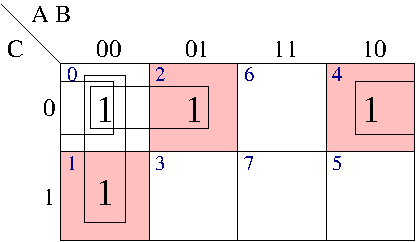
\includegraphics{../CombinationalCircuits/Assessments/wakerly_4_15_a}\\ \\
(b)\\
$F=\sum_{W,X,Y,Z}(1,4,5,6,11,12,13,14)=X \cdot Z' + W' \cdot Y' \cdot Z + X \cdot Y'+ W \cdot X' \cdot Y \cdot Z$\\
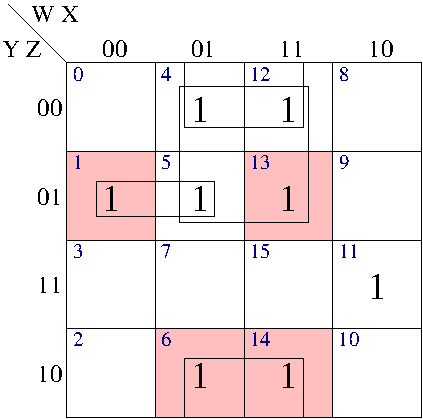
\includegraphics{../CombinationalCircuits/Assessments/wakerly_4_15_b}\\ \\
(c)\\
$F=\prod_{A,B,C}(1,2,6,7)=\sum_{A,B,C}(0,3,4,5)=B' \cdot C' + A \cdot B' + A' \cdot B \cdot C$\\
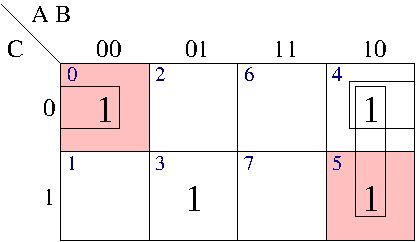
\includegraphics{../CombinationalCircuits/Assessments/wakerly_4_15_c}\\ \\
\end{minipage}\\
&\begin{minipage}[t]{\linewidth}
(d)\\
$F=\sum_{W,X,Y,Z}(0,1,2,3,7,8,10,11,15)=W' \cdot X' + Y \cdot Z + W \cdot X' \cdot Z'$\\
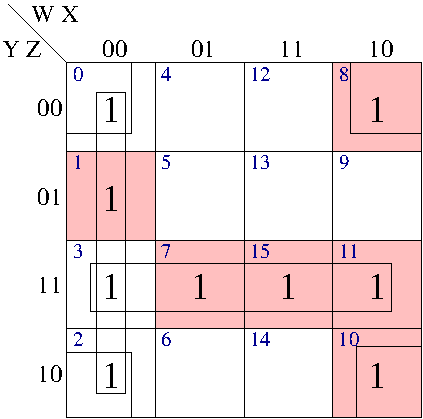
\includegraphics{../CombinationalCircuits/Assessments/wakerly_4_15_d}\\ \\
(e)\\
$F=\sum_{W,X,Y,Z}(1,2,4,7,8,11,13,14)=W' \cdot X' \cdot Y' \cdot Z + W' \cdot X' \cdot Y \cdot Z' + W' \cdot X \cdot Y' \cdot Z' + W' \cdot X \cdot Y \cdot Z + W \cdot X \cdot Y' \cdot Z + W \cdot X \cdot Y \cdot Z' + W \cdot X' \cdot Y' \cdot Z' + W \cdot X' \cdot Y \cdot Z$\\
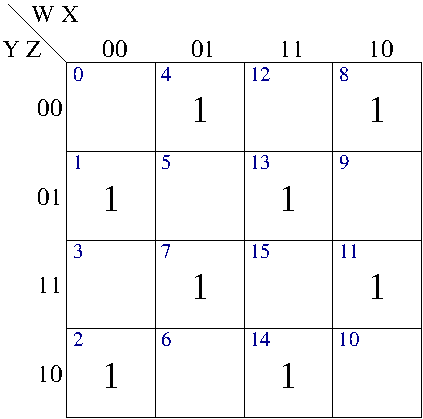
\includegraphics{../CombinationalCircuits/Assessments/wakerly_4_15_e}\\ \\
(f)\\
$F=\prod_{A,B,C,D}(1,3,4,5,6,7,9,12,13,14)=\sum_{A,B,C,D}(0,2,8,10,11,15)=B' \cdot D' + A \cdot C \cdot D$\\
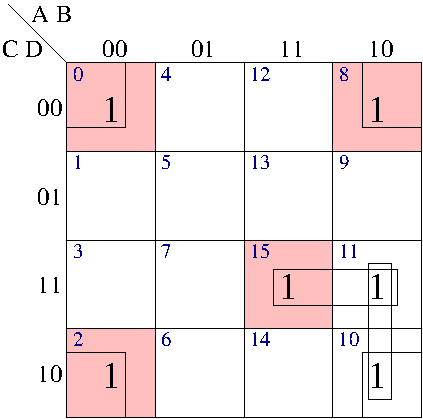
\includegraphics{../CombinationalCircuits/Assessments/wakerly_4_15_f}\\ \\
\end{minipage}\\
\medskip
%file: ../CombinationalCircuits/Assessments/wakerly_4_36.tex
5.&\begin{minipage}[t]{\linewidth}(4 pt) Do problem 4.36 in the text.\\ \\

Solution: \\ \\
\begin{tabular}{cc|c}
  $A$ & $B$ & $F$ \\
  \hline
   0  &  0  &  1 \\
   0  &  1  &  0 \\
   1  &  0  &  0 \\
   1  &  1  &  1 \\
\end{tabular}\\ \\
$F=\sum_{A,B}(0,3)=A' \cdot B' + A \cdot B$\\ \\
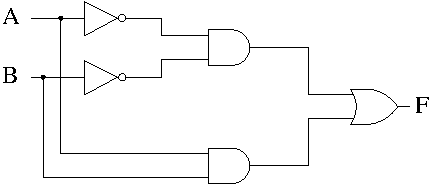
\includegraphics{../CombinationalCircuits/Assessments/wakerly_4_36}\\
\end{minipage}\\
\medskip
\end{longtable}
\end{document}
